\section{Manuel utilisateur}
\label{sec:manuel}

Bienvenue dans le manuel utilisateur de Glasir, un logiciel d'aide aux experts en sécurité basé sur le formalisme des ADTrees\footnote{Abréviation d'\og Attack-Defense Trees \fg{}, ou \og Arbres d'Attaque et de Défense\fg{} en français.}. Grâce à Glasir, vous pourrez analyser efficacement vos ADTrees préalablement créés avec ADTool~\cite{adtool}, un logiciel open-source disponible sur Internet.

Ce livret commencera par décrire le fonctionnement général du logiciel (création d'un nouveau projet, ouverture d'un projet existant, etc.), avant d'expliquer comment prendre en main les trois fonctionnalités principales que sont l'Éditeur de fonctions, le Filtre et enfin l'Optimiseur. 

Après cela, dans la {\sc sous-section}~\ref{ssec:manuelADTool} vous trouverez des détails concernant l'utilisation d'ADTool, surtout les nouveautés qui lui ont été ajoutées lors de ce projet.

\begin{figure}[!h]
        \centering
        
\includegraphics[height=0.3\textwidth]{figure/glasir.png}
    \end{figure}

\subsection{Glasir}
\label{ssec:manuelGlasir}

\paragraph{Fonctionnement général}

\paragraph{Éditeur de fonctions}Cette fonctionnalité a pour intérêt d'exprimer un compromis entre deux valuations d'un ADTree en en créant une troisième, fonction des deux premières. Par exemple, si vous avez un ADTree qui a comme paramètres \og Minimal cost for the proponent \fg (en euros) et \og Minimal time for the proponent (sequentiall) \fg (en heures) et que vous estimez que une heure \og coute \fg par comparaison 20 euros, vous pouvez créer un nouveau paramètre de type \og Minimal cost for the proponent \fg exprimant un compromis entre les deux paramètres qui sera égal à coût+20*temps.
Pour utiliser l'éditeur de onctions, suivez les étapes suivantes : 
\begin{itemize}
\item Assurer vous d'avoir l'ADTree que vous voulez utiliser d'ouvert et désigné comme l'arbre courant. 
\item Sélectionnez l'onglet \og FunctionEditor \fg .
\item Sélectionnez les deux paramètres de l'ADTree que vous voulez combiner au moyen des deux ComboBox présentent dans l'onglet. ATTENTION  ! : le nouveau paramètre aura pour type celui du premier paramètre sélectionné (à gauche), par exemple si le premier paramètre est de type \og Minimal time for the proponent (sequentiall) \fg , alors le nouveau paramètre calculé le sera aussi. Si vous sélectionnez un paramètre de type discret, un nombre de cases égal au nombre valeurs possibles s'affichera. Vous pourrez alors pondérer ces valeurs de la plus petite (à gauche), à la plus grande (à droite).
\item Inscrivez dans la textBox \og Function \fg la fonction que vous voulez utiliser pour le calcul du nouveau paramètre. Par exemple, si vous voulez faire \og newParam = firstParam + 2*secondParam\fg , inscrivez \og +2*\fg .
\item Entrez le nom que vous voulez donné au nouveau paramètre créé dans la textBox \og Name\fg.
\item Enfin, cliquez sur le bouton \og Apply\fg pour créer le nouveau paramètre.
\end{itemize} 
S'ouvrira alors un nouvel arbre dans une nouvelle fenêtre d'ADTool qui sera nommé comme l'arbre utilisé suivi de \og .functEdit\fg . Le nouvel arbre sera enregistré dans le répertoire où se trouve le logiciel Glasir. 
Si un problème survient, l'exécution sera interrompu et une boite de message apparaitra pour vous expliquer pourquoi.

\paragraph{Filtre}Cette fonctionnalité sert a élaguer les chemins d'un ADTree qui ne respectent pas une certaine condition. Par exemple si un ADTree a comme paramètre \og Minimal cost for the proponent \fg (en euros) et que l'on sait qu'un attaquant potentiel ne peut pas dépenser plus de 2000 euros, le filtre permettra alors d'élaguer l'ADTree de manière a ne conserver que les feuilles de l'arbre qui apparaissent dans au moins un chemin permettant d'accomplir l'attaque avec 2000 euros ou moins.
Pour utiliser le filtre, suivez les étapes suivantes :
\begin{itemize}
\item Assurer vous d'avoir l'ADTree que vous voulez filtrer d'ouvert et désigné comme l'arbre courant. 
\item Sélectionnez l'onglet \og Filter \fg .
\item Sélectionnez le paramètre selon lequel vous voulez filtre l'arbre avec la ComboBox présente dans l'onglet.
\item Indiquer dans la textBox \og Limit Value\fg la pire valeur acceptable par le filtre pour le paramètre sélectionné. Vous pouvez rentrez une valeur textuelle correspondant à l'une des valeurs de l'ensemble du paramètre si l'ensemble est discret.
\item Enfin, cliquez sur le bouton \og Filter\fg pour filtrer l'arbre.
\end{itemize}
S'ouvrira alors un nouvel arbre correspondant à l'arbre élagué dans une nouvelle fenêtre d'ADTool, qui sera nommé comme l'arbre utilisé suivi de \og .filter\fg . Le nouvel arbre sera enregistré dans le répertoire où se trouve le logiciel Glasir.
Si un problème survient, l'exécution sera interrompu et une boite de message apparaitra pour vous expliquer pourquoi.

\paragraph{Optimiseur}Cette fonctionnalité sert a élaguer les chemins d'un ADTree de manière a ne conserver que le ou les meilleurs chemins selon un paramètre donné. Par exemple si un ADTree a comme paramètre \og Minimal cost for the proponent \fg (en euros) et que l'attaque la moins chère coute 2000 euros, l'optimiseur permettra alors d'élaguer l'ADTree de manière a ne conserver que les feuilles de l'arbre qui apparaissent dans au moins un chemin permettant d'accomplir l'attaque avec 2000 euros seulement.
Pour utiliser l'optimiseur, suivez les étapes suivantes :
\begin{itemize}
\item Assurer vous d'avoir l'ADTree que vous voulez filtrer d'ouvert et désigné comme l'arbre courant. 
\item Sélectionnez l'onglet \og Optimize \fg .
\item Sélectionnez le paramètre selon lequel vous voulez optimiser l'arbre avec la ComboBox présente dans l'onglet.
\item Enfin, cliquez sur le bouton \og Optimize\fg pour filtrer l'arbre.
\end{itemize}
S'ouvrira alors un nouvel arbre correspondant à l'arbre élagué dans une nouvelle fenêtre d'ADTool, qui sera nommé comme l'arbre utilisé suivi de \og .Optimizer\fg . Le nouvel arbre sera enregistré dans le répertoire où se trouve le logiciel Glasir.
Si un problème survient, l'exécution sera interrompu et une boite de message apparaitra pour vous expliquer pourquoi.

\subsection{Nouvelles fonctionnalités d'ADTool}
\label{ssec:manuelADTool}

Pour le fonctionnement basique d'ADTool, vous pouvez vous référer au manuel utilisateur officiel disponible sur Internet\footnote{Voir à l'adresse suivante : http://satoss.uni.lu/members/piotr/adtool/manual.pdf}. Le guide ici présent ne détaillera que l'utilisation des nouvelles fonctionnalités d'ADTool, qui sont le copier/couper/coller ainsi que l'annulation d'une action.

\paragraph{Copier/couper/coller} Ces fonctionnalités vous seront utiles si vous désirez couper/copier un sous-arbre de l'ADTree courant afin de le coller ensuite à un autre emplacement dans ce même ADTree. Il est à noter que le sous-arbre coupé/copié sera ajouté en tant que fils du n\oe{}ud auquel il sera collé. Aussi, la racine du sous-arbre coupé/copié doit être du même type (opponent ou proponent) que son futur n\oe{}ud parent. Pour couper/copier un sous-arbre puis le coller, suivez les étapes suivantes : 
\begin{enumerate}
    \item Sélectionnez à l'aide d'un clic gauche le n\oe{}ud racine du sous-arbre que vous désirez couper/copier. Si vous avez déjà sélectionné un n\oe{}ud dans l'arbre, vous pouvez également vous déplacer jusqu'au n\oe{}ud souhaité à l'aide des flèches (haut, bas, gauche, droite) du clavier.
	\item Effectuez un clic droit sur le n\oe{}ud sélectionné. Un menu déroulant doit apparaître à côté du n\oe{}ud sélectionné, comme sur la {\sc Figure}~\ref{fig:clicdroit}.
	\item Sélectionnez l'option \og Copy Subtree \fg{}/\og Cut Subtree \fg{}) dans le menu déroulant. Vous pouvez également effectuer cette étape à l'aide d'un raccourci clavier, {\sc CTRL+C}/{\sc CTRL+X}.
	\item Effectuez un clic droit sur le n\oe{}ud auquel vous voulez coller le sous-arbre coupé/copié, puis sélectionnez dans la liste déroulante \og Paste Subtree as Child \fg{}. Si cette option n'apparaît pas dans le menu déroulant, c'est que vous n'avez pas préalablement coupé/copié de sous-arbre. Vous pouvez ici encore utiliser un raccourci clavier, {\sc CTRL+V}.
\end{enumerate}

    \begin{figure}[!h]
        \centering
        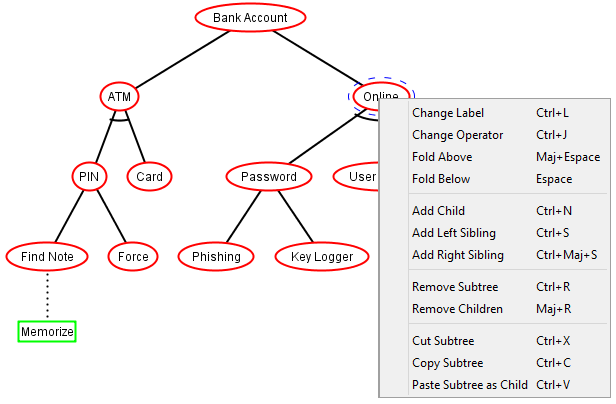
\includegraphics[height=0.7\textwidth]{figure/clicdroit.png}
        \caption{Menu déroulant apparaissant après un clic droit sur un n\oe{}ud.}
        \label{fig:clicdroit}
    \end{figure}

\paragraph{Annulation d'une action} Il s'agit ici d'annuler une ou plusieurs action(s) effectuée(s) précédemment sur l'ADTree courant. Pour cela, il vous suffit tout simplement d'utiliser le raccourci clavier {\sc CTRL+Z} autant de fois que nécessaire, jusqu'à retrouver l'état souhaité pour l'ADTree. Vous pouvez également cliquer sur l'icône \og Undo last action (CTRL+Z) \fg{} en haut à gauche de la fenêtre principale d'ADTool, encadrée en rouge sur la {\sc figure}~\ref{fig:undo}. Les actions pouvant être annulées sont les changements de labels, les ajouts ou suppressions de n\oe{}uds, les changements d'opérateur (conjonction ou disjonction) ainsi que les actions de couper/copier/coller.

\begin{figure}[!h]
        \centering
        
\includegraphics[height=0.17\textwidth]{figure/undo.png}
        \caption{Icône permettant d'annuler l'action précédente.}
        \label{fig:undo}
    \end{figure}